
\documentclass[conference]{IEEEtran}
\IEEEoverridecommandlockouts
\usepackage[T1]{fontenc}
\usepackage[utf8]{inputenc}
\usepackage{cite}
\usepackage{url}
\usepackage{booktabs}
\usepackage{array}
\usepackage{tabularx}
\usepackage{multirow}
\usepackage{graphicx}
\usepackage{xcolor}
\usepackage{balance}
\usepackage[hidelinks]{hyperref}

\hyphenation{low-code no-code citizen-development model-driven}

\begin{document}

\title{Low-Code and No-Code Platforms in Software Engineering: A PRISMA-Informed Review of Benefits, Challenges, and Future Directions}

\author{
\IEEEauthorblockN{Aman J Sonal, Deepak Naik, Chithra K}
\IEEEauthorblockA{
School of Computer Engineering\\
Manipal Institute of Technology, Manipal Academy of Higher Education\\
Manipal, India\\
\texttt{aman7.mitmpl2024@learner.manipal.edu},
\texttt{deepak.mitmpl2024@learner.manipal.edu},
\texttt{k.chithra@manipal.edu}
}
}


\maketitle

\begin{abstract}
Low-code and no-code (LCNC) platforms have moved from peripheral rapid-application tools to a visible part of contemporary software engineering, especially as visual modelling, citizen development, and generative AI begin to converge. This paper presents a PRISMA-informed review of LCNC research with emphasis on benefits, challenges, and future directions. The review was constructed from a 170-record evidence corpus assembled from author-supplied candidate papers and supplementary academic web searching, then screened to a final set of 50 included studies. Data extraction covered study metadata, method, platform or domain context, quality appraisal, evidence quotes, thematic codes, and synthesis notes. The strongest recurring themes were platform comparison and AI automation, while education, enterprise adoption, usability, integration, model-driven roots, and citizen development formed the next layer of evidence. Reported benefits include rapid prototyping, broader participation in software development, business-IT collaboration, education, and AI-assisted workflow generation. However, the same evidence base shows recurring concerns about governance, shadow IT, security and privacy, scalability, maintainability, platform lock-in, integration, testing, and the unclear boundary between citizen and professional development. To support auditability, the review links its synthesis to public extraction artifacts and a claim-to-evidence map. We conclude with a research agenda that prioritizes governance frameworks, security-by-design, maintainability benchmarks, interoperability, standardized evaluation metrics, and responsible human-AI collaboration.
\end{abstract}

\begin{IEEEkeywords}
Low-code development, no-code development, software engineering, citizen development, model-driven engineering, generative AI, systematic literature review.
\end{IEEEkeywords}

\section{Introduction}
Low-code and no-code platforms promise a pragmatic shift in how software is specified, implemented, and maintained. Instead of treating programming only as textual coding by professional developers, LCNC environments expose higher-level abstractions: visual models, forms, workflow builders, drag-and-drop components, templates, connectors, and increasingly natural-language interfaces. This shift is visible across open-source platform work and model-driven engineering \cite{p02,p20}, commercial platform studies \cite{p19,p29}, and AI-enabled application builders \cite{p37,p39}. It also changes the social organization of software work by making business users and domain experts \cite{p13,p14}, educators and analysts \cite{p28,p47}, and other non-professional developers \cite{p18,p49} active participants in application construction.

The LCNC literature has expanded quickly, but it is fragmented. Some studies examine adoption and governance in enterprise settings \cite{p12,p13,p14,p18}; others focus on technical artifacts such as BESSER, LLM4FaaS, workflow generators, zero-code IoT, no-code agents, and low-code AI platforms \cite{p01,p02,p04,p07,p31,p32,p35}. A third strand investigates developer experience, bugs, requirements engineering, platform interoperability, and the changing role of professional developers \cite{p23,p24,p26,p30,p34,p43,p46,p49}. Recent work further complicates the picture by connecting LCNC with large language models (LLMs) and generative UI tools \cite{p03,p06,p08,p22}, model-based consistency support \cite{p10,p33}, multi-agent systems \cite{p32,p40,p41}, and prompt-driven programming \cite{p11,p21,p42,p50}. These streams share an interest in raising abstraction, but they use different assumptions, evidence types, and terminology.

While recent systematic reviews have explored LCNC adoption patterns \cite{p18} and the general intersection of LCNC with AI \cite{p11}, this review distinguishes itself in three key ways. First, it specifically targets the rapid influx of 2024--2026 literature focusing on LLM-driven, agentic, and multimodal LCNC tools, which post-date prior reviews. Second, it integrates a quality appraisal of both technical prototypes and socio-technical governance studies, rather than focusing solely on one domain. Third, it translates the synthesis directly into a structured, actionable research agenda for software engineering practice, moving beyond descriptive mapping.

A systematic review is therefore needed for three reasons. First, claims about speed and democratization are often made beside warnings about security, maintainability, and vendor lock-in; a balanced synthesis is needed to prevent either promotional or dismissive accounts of LCNC adoption \cite{p15,p18,p26,p30,p34}. Second, the evidence base spans technical evaluations, surveys, interviews, focus groups, case studies, and prior reviews, making quality-sensitive interpretation necessary. Third, AI-assisted LCNC is changing quickly: LLMs can generate workflows or code from natural language, but the reliability of generated artifacts, the design of human handoff, and the governance of AI-generated applications remain unsettled \cite{p04,p05,p07,p08,p31,p41,p42}.

This review makes four contributions. First, it provides a PRISMA-informed account of how a 170-record LCNC corpus was screened to 50 included studies. Second, it synthesizes reported benefits and challenges using a coded extraction and quality appraisal. Third, it maps dominant research methods, themes, platform types, and domains. Fourth, it develops a future research agenda for LCNC software engineering, with special attention to generative AI and responsible citizen development.

Table~\ref{tab:related} positions this work against closely related reviews. The distinction is important because this paper is not intended to replace prior LCNC reviews. Instead, it extends them with a recent AI-era corpus, an explicit quality-appraisal summary, public extraction artifacts, and a synthesis that treats technical prototypes and socio-technical adoption studies together.

\begin{table*}[t]
\centering
\caption{Positioning Against Closely Related LCNC Reviews}
\label{tab:related}
\scriptsize
\begin{tabularx}{\textwidth}{p{0.16\textwidth} p{0.18\textwidth} p{0.18\textwidth} p{0.40\textwidth}}
\toprule
Review & Primary scope & Evidence emphasis & Difference from this paper \\
\midrule
Ajimati et al. \cite{p18} & Adoption of low-code/no-code development. & Adoption patterns and future research agenda. & Adds recent AI-era systems and quality appraisal. \\
Liwanag et al. \cite{p11} & LCNC development in the era of artificial intelligence. & Intersection of LCNC and AI. & Adds governance, quality, and extraction evidence. \\
Rokis and Kirikova \cite{p29} & Broad low-code development literature. & Conceptual and platform-oriented literature review. & Adds recent 2024--2026 synthesis and theme mapping. \\
Trieflinger et al. \cite{p15} & Potentials and risks of low-code development. & Benefits and risk profile from an SLR. & Adds LLM-era evidence and explicit risk-gap framing. \\
\bottomrule
\end{tabularx}
\end{table*}

\section{Background}
\subsection{Low-Code and No-Code Development}
Low-code development generally refers to software creation through higher-level abstractions that reduce the amount of hand-written code required, while still allowing custom logic, extension, and developer intervention. No-code development aims to move further toward configuration, composition, templates, and natural-language or visual interaction so that non-programmers can produce executable systems with little or no textual coding \cite{p02,p04,p19,p29}. The boundary is not fixed: platforms often contain both low-code and no-code features, and the same environment may be no-code for simple tasks but low-code once integration, testing, security, or customization is required \cite{p22,p34,p49}.

\subsection{Citizen Development and Professional Software Engineering}
Citizen development describes application creation by employees or domain specialists who are not formally trained as software engineers. In enterprise settings, LCNC is often presented as a way to reduce development backlogs, speed process digitization, and make business knowledge directly actionable \cite{p13,p14,p16,p18}. Yet the literature also shows that citizen development does not remove the need for professional software engineering. Professional developers remain central for architecture, integration, quality assurance, security, complex change management, and platform governance \cite{p30,p32,p43,p47,p49}.

\subsection{Model-Driven, Visual, and AI-Assisted Roots}
LCNC is not an isolated trend. It inherits ideas from model-driven engineering, visual programming, end-user development, domain-specific languages, workflow modelling, and rapid application development \cite{p20,p29,p33,p43}. The current wave differs because AI is becoming an active development participant. LLMs are now used to generate functions, workflows, explanations, UI code, IoT trigger-action rules, agent configurations, and domain-specific application logic from natural-language prompts \cite{p04,p05,p07,p08,p31,p35,p39,p40}. This creates opportunities for broader participation, but it also raises software engineering questions about correctness, reproducibility, traceability, and human oversight.

\section{Research Questions}
The review addresses five research questions:

\textbf{RQ1:} What benefits of LCNC platforms are reported in software engineering research?

\textbf{RQ2:} What technical, organizational, security, governance, and maintainability challenges are reported?

\textbf{RQ3:} What research methods, domains, and platform types dominate the LCNC literature?

\textbf{RQ4:} How are AI and generative AI reshaping LCNC development?

\textbf{RQ5:} What future research directions emerge from the reviewed studies?

\section{Methodology}
\subsection{Review Design}
The review followed a PRISMA-informed review workflow rather than a fully registered PRISMA 2020 protocol. This distinction is important. The corpus was constructed systematically and documented in project spreadsheets, per-paper JSON files, and extraction workbooks, but the protocol was not preregistered and database-native export logs were not preserved for every search source. The method is therefore described throughout as a PRISMA-informed review, not as a fully reproducible registered PRISMA review. To reduce ambiguity, the repository now contains the completed extraction workbook, PDF manifests, per-paper JSON outputs, a search/reproducibility log, per-paper quality appraisal CSV, evidence quote CSV, theme matrix CSV, and a working PRISMA checklist table.

\subsection{Search Strategy and Sources}
The starting corpus consisted of author-supplied candidate-paper spreadsheets and a previously curated shortlist. A supplementary search was conducted on 12 June 2026 across publisher pages, open repositories, and academic indexing surfaces, including arXiv, ACM and ACL Digital Library, SpringerLink, IEEE Xplore, MDPI, Wiley, AIS eLibrary, Google Scholar, and institutional repositories. 

The supplementary search used structured Boolean strings designed to capture the intersection of LCNC platforms with recent AI advancements and software engineering challenges. The base strings were:

\begin{itemize}
    \item \textbf{S1 (LCNC and AI Intersection):} \texttt{("low-code" OR "no-code" OR "citizen development") AND ("LLM" OR "generative AI" OR "automation")}
    \item \textbf{S2 (AI-Assisted Workflows):} \texttt{("low-code" OR "no-code") AND ("workflow" OR "prompt" OR "agent" OR "IoT")}
    \item \textbf{S3 (Engineering Challenges):} \texttt{("low-code" OR "no-code") AND ("governance" OR "security" OR "maintainability")}
\end{itemize}

These base strings were adapted to the syntax requirements of each source where possible. However, exact database-native query exports, hit counts, and timestamps were not retained for every source. This is now treated as a reproducibility limitation rather than hidden behind the review label. The available evidence package preserves the final 170-record corpus, the final top-50 selection, the extraction workbook, and the generated supplementary CSV files. The supplementary search intentionally emphasized recent work from 2024--2026 because generative AI is rapidly changing the LCNC research landscape, and older literature does not adequately cover LLM-driven development.

\begin{table}[t]
\centering
\caption{Search Transparency and Reproducibility Status}
\label{tab:searchlog}
\scriptsize
\begin{tabularx}{\columnwidth}{p{0.27\columnwidth}X}
\toprule
Item & Status in this revision \\
\midrule
Search date & 12 June 2026, recorded in project artifacts. \\
Starting records & 125 author-supplied records plus 45 supplementary records. \\
Search strings & Base Boolean strings S1--S3 reported in the manuscript. \\
Database-specific hit logs & Not fully preserved; disclosed as a limitation. \\
Screening artifacts & 170-record workbook, final top-50 list, PDF manifest, and extraction workbook. \\
Supplementary files & Per-paper quality appraisal, evidence quotes, theme matrix, claim-to-evidence map, and PRISMA checklist working table. \\
\bottomrule
\end{tabularx}
\end{table}

\subsection{Screening and Eligibility}
Fig.~\ref{fig:prisma} summarizes the screening flow. The corpus contained 170 records: 125 records from the initial candidate material and 45 additional records from the supplementary search. Nine records were flagged before screening as duplicates, low-fit, blog-like, or insufficiently research-oriented. The remaining 161 records were screened by title, abstract, metadata, source quality, full-text or article-page availability, and relevance to LCNC, citizen development, model-driven low-code engineering, AI-assisted no-code development, and software-engineering practice. Fifty studies were selected for the final synthesis, and 111 screened records were excluded after title/abstract/metadata or full-text relevance assessment. Thus, 120 records in total were not included in the final 50-paper review: nine flagged before screening and 111 excluded after screening. This resolves the apparent 111-versus-120 count ambiguity in earlier drafts.

\begin{figure*}[t]
\centering
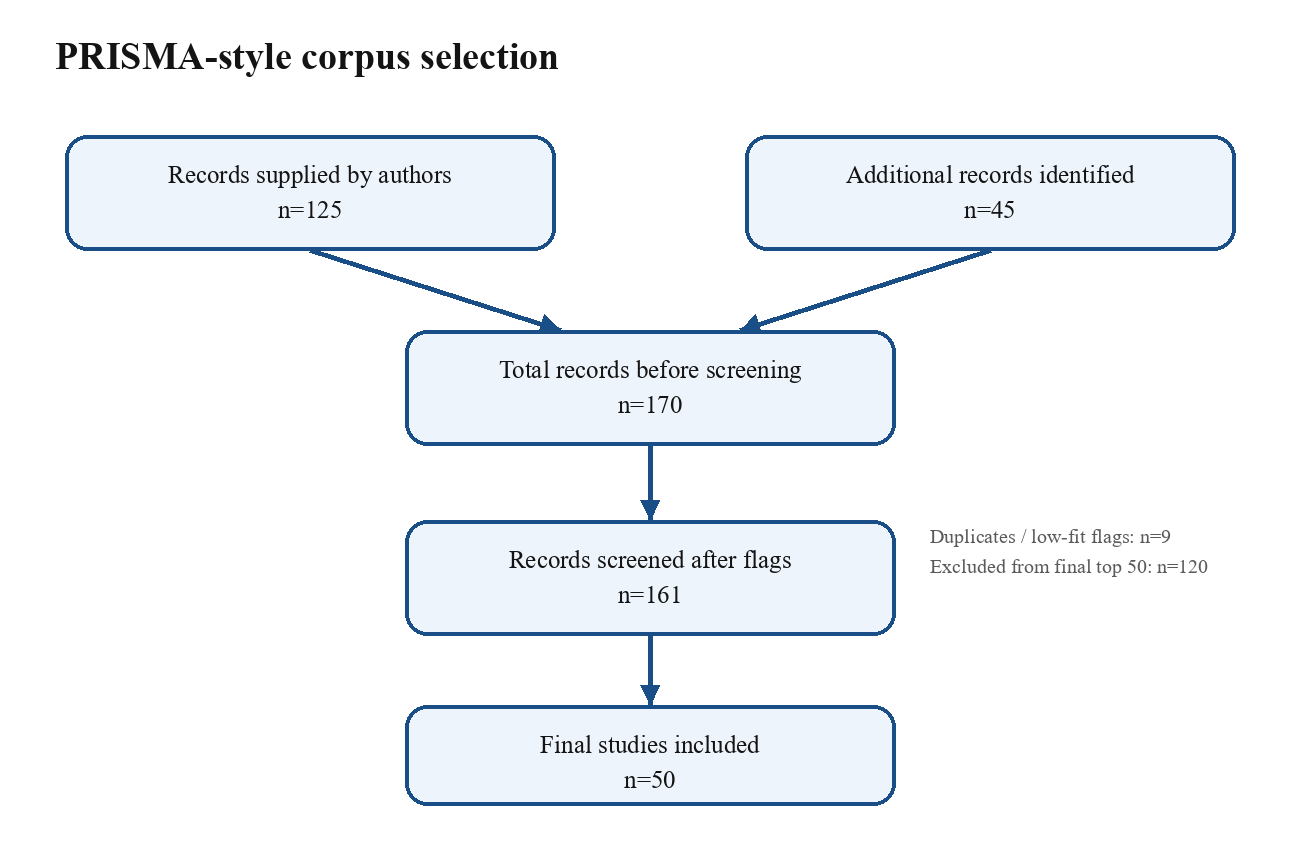
\includegraphics[width=0.82\textwidth]{figures/fig1_prisma_flow.png}
\caption{PRISMA-informed screening flow from 170 candidate records to 50 included studies.}
\label{fig:prisma}
\end{figure*}

\begin{table}[t]
\centering
\caption{Inclusion and Exclusion Criteria}
\label{tab:criteria}
\scriptsize
\begin{tabularx}{\columnwidth}{p{0.19\columnwidth}X}
\toprule
Type & Criteria \\
\midrule
Include & Research-oriented studies on LCNC, low-code, no-code, zero-code, citizen development, model-driven low-code, or AI-assisted LCNC. \\
Include & Papers with article page, PDF, repository copy, or sufficiently reliable metadata. \\
Include & Studies contributing to benefits, challenges, methods, platform design, AI automation, governance, or software-engineering implications. \\
Exclude & Blog posts, vendor-only white papers, duplicates, weak venue signals, inaccessible records with insufficient metadata, or weak LCNC relevance. \\
Exclude & Records whose contribution was too peripheral to support one of the review questions. \\
\bottomrule
\end{tabularx}
\end{table}

\subsection{Data Extraction and Coding}
The final 50 studies were extracted using a master schema covering bibliographic metadata, LCNC definitions, related terms, study object, research type, method, data source, sample or unit of analysis, domain, platform or tool, findings, limitations, implications, evidence strength, and future work. Evidence quotes were stored separately to support traceability from synthesis claims to paper-level evidence. The initial coding scheme identified 22 granular codes, which were iteratively consolidated into primary synthesis themes, including citizen development, productivity, governance, security and privacy, scalability, maintainability, lock-in, integration, usability, education, AI automation, quality assurance, domain-specific use, platform comparison, model-driven roots, and limitations. Table~\ref{tab:extraction} summarizes the extraction fields.

To improve transparency, this revision exports the extraction data as supplementary CSV files: per-paper extraction summaries, 200 evidence quote rows, a theme synthesis matrix, and a claim-to-evidence map. The screening and data extraction were primarily conducted by the first author, with a subset independently checked by another reviewer. Because a complete second-pass extraction and formal Cohen's kappa calculation were not performed, this manuscript no longer claims formal inter-rater reliability. Instead, the limitation is stated explicitly and the underlying evidence artifacts are made available for audit.

\begin{table}[t]
\centering
\caption{Data Extraction Fields}
\label{tab:extraction}
\scriptsize
\begin{tabularx}{\columnwidth}{p{0.30\columnwidth}X}
\toprule
Category & Examples of extracted fields \\
\midrule
Metadata & Paper ID, title, authors, year, venue, URL, access status. \\
Concepts & Definitions of low-code/no-code, related terms, scope conditions. \\
Method & research type, design, data type, sample, instruments, analysis technique. \\
Evidence & main findings, benefits, challenges, limitations, quotes, statistics. \\
Themes & up to four theme codes per paper plus section-use guidance. \\
Quality & 12 appraisal questions, total score out of 24, rating, risk notes. \\
\bottomrule
\end{tabularx}
\end{table}

\subsection{Quality Appraisal}
Each included study was scored on 12 criteria: clarity of aim, method fit, sample/data adequacy, context clarity, analytical rigor, validity or reliability checks, evidence-claim alignment, limitations, LCNC relevance, novelty, reproducibility/transparency, and usefulness for the review. Each criterion was evaluated on a three-point scale (0 = No, 1 = Partially, 2 = Yes), yielding a maximum possible score of 24. Stronger claims in this paper rely primarily on studies rated strong, while moderate studies are used cautiously as supporting or illustrative evidence. To address scoring transparency, the full per-paper appraisal table is provided as \texttt{paper\_outputs/supplementary/per\_paper\_quality\_appraisal.csv}. The appraisal is still treated as a structured first-pass assessment rather than a substitute for expert manual review.

\section{Descriptive Overview of Included Studies}
The final set is recent: five studies are from 2026, 22 from 2025, 18 from 2024, four from 2023, and one from 2022. This distribution reflects the deliberate emphasis on the AI-era LCNC literature, but it also means that some evidence is based on preprints, demonstrations, or fast-moving conference work.

\begin{table}[t]
\centering
\caption{Study Distribution by Year}
\label{tab:years}
\scriptsize
\begin{tabular}{lrrrrr}
\toprule
Year & 2022 & 2023 & 2024 & 2025 & 2026 \\
\midrule
Studies & 1 & 4 & 18 & 22 & 5 \\
\bottomrule
\end{tabular}
\end{table}

The method profile is mixed (Table~\ref{tab:methods}). Prototype evaluations and surveys are the largest identified method categories, followed by case studies and systematic reviews. Ten studies utilized hybrid approaches or did not explicitly label their primary method in the abstract, making strict single-category classification difficult; however, all 50 studies provided sufficient methodological detail in their full text to undergo quality appraisal.

\begin{table}[t]
\centering
\caption{Research Method Taxonomy}
\label{tab:methods}
\scriptsize
\begin{tabularx}{\columnwidth}{l r X}
\toprule
Method & Count & Typical contribution \\
\midrule
Prototype evaluation & 8 & Tool or platform behavior, usability, feasibility. \\
Survey & 8 & Perceptions, barriers, platform use, practitioner issues. \\
Case study & 6 & Contextual implementation or domain experience. \\
Systematic review & 5 & Prior evidence maps and research agendas. \\
Experiment & 3 & Task performance, feasibility, user outcomes. \\
Interview & 3 & Governance, process, role, developer experience. \\
Document analysis & 3 & Platform documentation or artifact review. \\
Benchmarking & 2 & Comparative performance or task evaluation. \\
Focus group & 1 & Stakeholder judgement of emerging approaches. \\
Literature review & 1 & Broad conceptual synthesis. \\
Not clearly reported & 10 & Method not extractable with enough confidence. \\
\bottomrule
\end{tabularx}
\end{table}

Quality appraisal was generally high, with 43 studies rated strong and seven moderate. The average score was 21.38 out of 24, but this should not be read as a guarantee that every claim is equally mature. This high average reflects clear aims, LCNC relevance, and usable evidence across the corpus. A study could score highly on analytical rigor and evidence-claim alignment even if its primary method was hybrid or unclassified (as noted in Table~\ref{tab:methods}); deductions were primarily applied for limited sample details, lack of external validity, or incomplete reproducibility, rather than an absence of methodological description.

\begin{table}[t]
\centering
\caption{Quality Appraisal Summary}
\label{tab:quality}
\scriptsize
\begin{tabularx}{\columnwidth}{l r X}
\toprule
Metric & Value & Interpretation \\
\midrule
Average score & 21.38/24 & High overall appraisal, with caution for automated extraction. \\
Strong studies & 43 & Main basis for synthesis claims. \\
Moderate studies & 7 & Used cautiously or illustratively. \\
Weak studies & 0 & No included study was coded weak. \\
Main caveat & -- & Some sample, metadata, and method fields were incomplete. \\
\bottomrule
\end{tabularx}
\end{table}

Theme coding shows that platform comparison and AI automation dominate the corpus, followed by education, enterprise adoption, usability, integration, model-driven roots, citizen development, governance, scalability, and quality testing (Table~\ref{tab:themes}). This profile suggests a field currently organized around platform capability and AI augmentation, with socio-technical governance and long-term engineering quality present but less densely evidenced.

\begin{table*}[t]
\centering
\caption{Theme Frequency Summary Across Included Studies (MDE: Model-Driven Engineering).}
\label{tab:themes}
\scriptsize
\begin{tabularx}{\textwidth}{l r X l r X}
\toprule
Theme & Count & Interpretation & Theme & Count & Interpretation \\
\midrule
Platform comparison & 40 & Tool features and platform capability dominate. &
AI and automation & 34 & LLM and agent support is a central recent theme. \\
Education/training & 18 & LCNC is linked to upskilling and beginner access. &
Enterprise adoption & 15 & Organizational adoption is a major concern. \\
Usability/UX & 13 & Ease of use is studied but remains context-dependent. &
Integration & 12 & API, data, and enterprise-system fit are recurring issues. \\
MDE/visual roots & 11 & LCNC remains connected to model-driven engineering. &
Citizen development & 10 & Non-professional development is a core social shift. \\
Governance & 7 & Oversight and control are central but under-specified. &
Scalability & 6 & Enterprise readiness and long-running agents need more evidence. \\
Quality/testing & 6 & Correctness and verification are emerging priorities. &
Professional role & 5 & LCNC changes, but does not remove, developer work. \\
Maintainability & 4 & Long-term evolution is a persistent concern. &
Domain-specific use & 4 & Agriculture, science, public-sector, and industrial examples appear. \\
Vendor lock-in & 3 & Portability and migration are still under-studied. &
Security/privacy & 2 & Important but thinly evidenced in the final set. \\
\bottomrule
\end{tabularx}
\end{table*}

Table~\ref{tab:claimmap} adds a compact claim-to-evidence bridge for the main synthesis claims. The full supporting file is exported as \texttt{claim\_to\_evidence\_map.csv}; detailed paper-level evidence remains in the evidence-quote supplement.

\begin{table*}[t]
\centering
\caption{Claim-to-Evidence Map for Central Synthesis Claims}
\label{tab:claimmap}
\scriptsize
\begin{tabularx}{\textwidth}{p{0.27\textwidth} p{0.20\textwidth} p{0.22\textwidth} X}
\toprule
Synthesis claim & Primary themes & Supporting papers & Evidence interpretation \\
\midrule
LCNC can accelerate bounded prototyping and workflow creation. & Productivity, platform comparison, AI automation & \cite{p04,p07,p18,p29,p31,p35,p46,p48} & Supported by prototype, review, requirements, workflow, and domain studies; strongest for bounded tasks and platform-supported domains. \\
Citizen development broadens participation but does not remove professional engineering responsibilities. & Citizen development, enterprise adoption, professional role, governance & \cite{p12,p13,p16,p18,p30,p47,p49} & Supported by enterprise, adoption, role, and developer-discussion evidence; requires governance and escalation paths. \\
Security and privacy are high-impact but under-represented. & Security/privacy, governance, quality testing & \cite{p15,p26,p28,p30} & Treated as an evidence gap, not as a high-frequency finding; only two papers were primarily coded security/privacy. \\
AI-assisted LCNC shifts development toward prompt-, agent-, and workflow-mediated specification. & AI automation, MDE/visual roots, usability & \cite{p04,p05,p06,p07,p08,p31,p32,p35,p40,p41,p42,p50} & Supported by recent prototype, benchmark, agent, workflow, and user-study papers; rapidly evolving evidence. \\
Maintainability, scalability, portability, and lifecycle governance remain less mature evidence areas. & Maintainability, scalability, vendor lock-in, integration, governance & \cite{p12,p14,p15,p26,p29,p30,p34,p41,p49} & Supported mainly as recurring limitations and future-work needs rather than settled empirical conclusions. \\
\bottomrule
\end{tabularx}
\end{table*}

Fig.~\ref{fig:taxonomy} presents the synthesis framework used in the remainder of the paper. LCNC value is produced when abstraction, automation, and participation are balanced against governance, quality, and long-term maintainability.

\begin{figure*}[t]
\centering
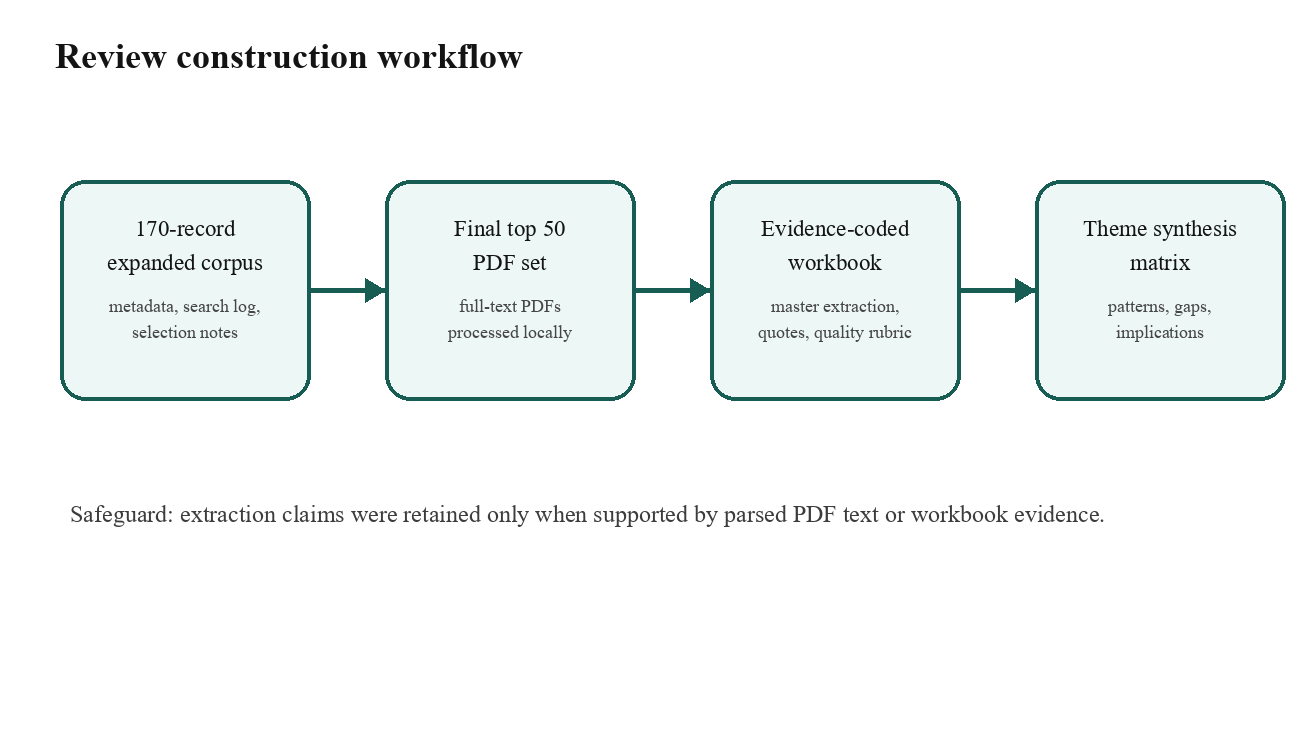
\includegraphics[width=0.86\textwidth]{figures/fig2_workflow.png}
\caption{Extraction-to-synthesis workflow used to convert the PDF corpus and extraction workbook into review themes, claim evidence, quality appraisal, and future directions.}
\label{fig:taxonomy}
\end{figure*}

\section{Thematic Synthesis: Benefits}
\subsection{Faster Development and Prototyping}
The most frequently reported benefit is acceleration in bounded development tasks. LCNC platforms reduce boilerplate, provide reusable components, and support rapid iteration, which is especially useful when requirements are understood but developer capacity is limited \cite{p18,p29,p46,p48}. Technical studies extend this claim to AI-enabled pipelines. LLM4FaaS illustrates how natural-language requirements can be transformed into deployable serverless functions under controlled conditions, reducing the operational burden associated with code generation and deployment \cite{p04}. Workflow-generation research similarly investigates whether smaller fine-tuned models or prompted LLMs can produce structured low-code workflows, making development speed a measurable AI-assisted outcome rather than a purely managerial claim \cite{p07}. Zero-code IoT and no-code workflow-builder studies show similar movement toward natural-language specification of executable behavior \cite{p31,p35}.

This benefit should be interpreted carefully. Faster artifact generation is strongest when tasks are bounded, platforms provide suitable abstractions, and the generated system remains within the platform's intended domain. Studies of feature addition, IoT applications, and process modelling show that speed does not remove the need for verification, domain review, and iteration \cite{p05,p08,p35,p43}.

\subsection{Democratization and Citizen Development}
LCNC expands who can participate in software creation. Enterprise citizen developer programs report that business users can contribute domain knowledge more directly, improving alignment between software artifacts and business processes \cite{p13,p18}. Multisector adoption work frames LCNC as part of digital transformation because it enables non-IT groups to prototype and deploy process-specific applications \cite{p14}. Practical and domain-oriented studies in research applications, precision agriculture, AI tools, and XAI also show that non-experts can build or use computational tools when interaction is visual, configured, or guided by natural language \cite{p28,p37,p48,p50}.

The democratization claim is not a claim that programming expertise becomes unnecessary. Rather, the evidence suggests a redistribution of work. Citizen developers gain local autonomy for simpler workflows, while professional developers and platform specialists become responsible for enabling reusable components, integration, quality gates, governance models, and escalation paths \cite{p16,p30,p47,p49}.

\subsection{Business-IT Collaboration and Digital Transformation}
LCNC can act as a boundary object between business and IT. HICSS evidence on enterprise citizen developer programs emphasizes business-IT collaboration as a central adoption mechanism, while standardization research shows that flexibility must be balanced with organizational control \cite{p12,p13}. Adoption and SLR studies similarly associate LCNC with digital transformation, process improvement, and organizational experimentation \cite{p14,p18}. The practical value lies not only in faster implementation, but in shorter feedback cycles between process owners and technical teams.

This collaborative benefit is strongest when platforms are embedded in a clear operating model. Without defined ownership, review, and lifecycle responsibilities, the same flexibility that supports innovation can produce ungoverned applications and fragmented digital processes \cite{p12,p15,p18}.

\subsection{Education, Training, and Skill Development}
Eighteen studies were coded to education and training, making this one of the most frequent themes. LCNC and no-code ML tools can lower barriers for learners who need to understand computational thinking, ML workflows, AI pipelines, or domain automation without first mastering full-scale programming environments \cite{p19,p28,p37,p39}. AI-assisted end-user development, ChatGPT-supported no-code exploration, and no-code explainability work suggest that natural-language and visual tools can support novice comprehension when explanations, feedback, and task structure are designed carefully \cite{p27,p44,p50}. Robotics, localization, and AI-for-science studies extend this educational value to domain experts who need executable artifacts but do not identify as professional software developers \cite{p01,p36,p45}.

However, education should not be reduced to tool operation. Several studies imply that users also need conceptual training in requirements, data quality, security, testing, and responsible use \cite{p16,p26,p30,p46}. LCNC curricula should therefore teach both how to build with platforms and how to reason about the software engineering consequences of what is built.

\subsection{AI-Assisted Workflow Generation and Automation}
AI is now central to LCNC research. LLMs support no-code serverless development, IoT applications, decision-rule prompting, workflow generation, feature addition, multi-agent configuration, and multimodal no-code systems \cite{p04,p05,p06,p07,p08,p31,p32,p40}. AI can help users move from intent to executable structure by extracting data, actions, context, rules, and workflow components \cite{p31,p35}. It can also act as an assistant inside low-code AI-development environments, where visual programming and code-generation support complement each other \cite{p39}.

The strongest AI-related evidence remains mixed in scope. Benchmarks and prototypes show feasibility, but many systems are task-specific and evaluated on constrained datasets or user studies \cite{p01,p08,p31,p50}. The implication is that AI-assisted LCNC is promising, but it should be evaluated as software engineering infrastructure rather than as a generic productivity shortcut.

\section{Thematic Synthesis: Challenges}
\subsection{Governance, Shadow IT, and Standardization}
The central organizational challenge is the tension between flexibility and control. LCNC empowers local innovation, but enterprise systems require standards for ownership, review, data access, deployment, monitoring, and retirement \cite{p12,p13,p15}. Governance research shows that standardization cannot simply suppress flexibility; it must define where citizen development is appropriate and where professional engineering review is mandatory \cite{p12}. Adoption studies similarly warn that LCNC becomes risky when applications are created outside official oversight or without lifecycle accountability \cite{p14,p18}.

Governance is especially important for AI-enabled LCNC. Natural-language interfaces and agents can make application creation even easier, which raises the risk that users generate workflows whose behavior they cannot fully inspect, test, or maintain \cite{p06,p31,p32,p42}. Future governance models must therefore cover both traditional platform artifacts and AI-generated or AI-mediated artifacts.

\subsection{Security, Privacy, and Compliance}
Security and privacy appear less frequently in the coded final set than platform comparison or AI automation, but they remain high-impact concerns. Practical reviews and developer-discussion studies identify access control, data exposure, authentication, platform infrastructure, and compliance as recurring issues in LCNC settings \cite{p28,p30}. These risks intensify when citizen developers connect enterprise data sources, third-party APIs, or AI services without a mature understanding of threat models and data governance.

The limited number of security-coded studies should not be interpreted as low risk; it indicates an evidence gap. LCNC applications often handle operational data, customer records, workflow approvals, or AI-generated content. Therefore, the absence of dense security evidence is itself a reason for future research in security-by-design, static analysis of low-code artifacts, permission modelling, and compliance-aware templates.

\subsection{Scalability, Performance, and Reliability}
Scalability concerns take several forms. Enterprise LCNC applications must handle growing data volumes, users, integrations, and business-critical workflows. AI-assisted LCNC systems introduce further scalability issues around prompt length, model selection, context limits, memory, latency, and cost \cite{p05,p38,p41}. Empirical bug research shows that low-code platforms are still software systems with reliability problems that can affect application behavior, platform components, and developer productivity \cite{p26}. Long-running low-code agents create a newer reliability challenge: maintaining contextual consistency over extended tasks \cite{p41}.

The literature does not support a blanket claim that LCNC platforms are either scalable or unscalable. Rather, scalability depends on the platform architecture, extension points, deployment model, integration style, and quality of generated or configured artifacts \cite{p18,p20,p26,p45}. This makes benchmarking and transparent performance reporting essential.

\subsection{Maintainability and Technical Debt}
Rapid composition can create technical debt when applications evolve beyond their original scope. Maintainability concerns include hidden logic, weak version control, limited testability, undocumented workflows, dependence on platform-specific abstractions, and difficulty changing applications once they become operationally important \cite{p14,p29,p30}. Open-source low-code platform work argues that extensibility and transparency matter because proprietary closed environments can make long-term maintenance and adaptation harder \cite{p02,p20}.

Maintainability is not only a technical property. It is also an organizational property: someone must own the artifact, understand its dependencies, test changes, and decide when to refactor, migrate, or retire it. This ownership question becomes sharper for citizen-developed applications and AI-generated workflows \cite{p13,p47,p49}.

\subsection{Vendor Lock-In, Portability, and Interoperability}
Vendor lock-in is a recurring risk in LCNC because many platforms use proprietary models, connectors, hosting services, and component libraries. Interoperability work shows that exporting and importing models across low-code platforms can lose elements or produce incorrect mappings \cite{p34}. Tool-review and professional-developer studies also identify migration difficulty and ecosystem dependence as barriers to strategic adoption \cite{p09,p49}. The implication is that LCNC portability should be treated as a software engineering requirement, not an afterthought.

Open-source and model-driven approaches provide partial responses. BESSER-related studies and interoperability research suggest that explicit models, transformations, and open platform architectures may reduce lock-in, but these approaches still require mature standards and empirical validation across platforms \cite{p02,p20,p34}.

\subsection{Integration, Testing, and Quality Assurance}
Integration is one of the most common non-AI themes. LCNC applications frequently need to connect databases, APIs, enterprise systems, IoT devices, ML services, or agent tools \cite{p17,p20,p30,p32,p40,p48}. Integration failures can undermine the very productivity gains that LCNC promises. Testing is equally important. Benchmarking, DevOps-oriented review work, and reliability studies show the need to evaluate generated features, workflows, code quality, syntax validity, semantic correctness, and platform bugs \cite{p04,p08,p21,p25,p26}. AI-for-science and metacognitive-agent studies further show that testing AI-generated artifacts requires more than standard unit tests; systems may need adversarial evaluation, uncertainty reduction, or explicit human handoff when failure is likely \cite{p01,p42}.

The synthesis therefore supports a cautious but important conclusion: LCNC does not reduce the importance of software quality assurance; it changes where and how assurance must occur.

\section{AI, Generative AI, and the Future of LCNC}
Generative AI is reshaping LCNC in three ways. First, it changes the input modality. Instead of requiring users to manipulate every visual element, LLM-supported tools allow natural-language descriptions of serverless functions, IoT trigger-action programs, workflows, process rules, or application features \cite{p04,p05,p07,p08,p35}. Second, it changes the artifact boundary. Generated output may be code, JSON workflow definitions, UI structures, agent configurations, decision rules, or explanations rather than a conventional source file \cite{p06,p31,p32,p39,p40}. Third, it changes responsibility. Users may specify intent, the AI may synthesize artifacts, and the platform may execute or deploy them; accountability for correctness must therefore be shared among users, platform designers, and software engineers.

Recent studies show both opportunity and risk. No-code agent tools and multimodal no-code systems make complex AI applications more accessible \cite{p32,p40}. AIAP and ChatIoT suggest that natural-language systems can help non-experts construct workflows or IoT programs \cite{p31,p35}. LLM4FaaS and workflow-generation studies show that deployment and workflow synthesis can be automated under controlled conditions \cite{p04,p07}. NoCode-bench begins to provide evaluation infrastructure for natural-language-driven feature addition \cite{p08}. At the same time, LLM suitability depends on model choice, prompt language, task complexity, and generated-application quality \cite{p05}. Low-code agents must manage memory and context across long tasks \cite{p41}. Failure prediction and human handoff become design requirements, not optional usability features \cite{p42}. No-code XAI studies suggest that explaining AI behavior without code is feasible for novices, but it must be designed and evaluated carefully \cite{p50}.

These findings suggest that AI-assisted LCNC should be treated as a new layer of software engineering automation. It needs requirements engineering, evaluation metrics, versioning, provenance, testing, and governance. The future question is not whether LLMs can generate LCNC artifacts, but under what conditions those artifacts can be trusted, maintained, integrated, audited, and safely handed back to humans.

\section{Discussion}
\subsection{The Core Trade-Off}
The review identifies a persistent trade-off: LCNC increases accessibility and speed by raising abstraction, but higher abstraction can hide complexity. Users gain faster construction, but they may lose visibility into generated logic, platform constraints, integration dependencies, performance limits, and security implications. This trade-off appears across enterprise adoption, no-code AI tools, interoperability research, and professional-developer studies \cite{p12,p18,p34,p39,p49}.

The field should therefore move beyond asking whether LCNC is good or bad. A better question is: for which tasks, users, governance arrangements, and quality requirements is LCNC appropriate? Simple departmental workflows, prototypes, educational tools, dashboards, and bounded AI services may be strong candidates. Regulated, safety-critical, high-scale, or deeply integrated systems need stronger professional oversight, formal testing, and governance.

\subsection{Implications for Software Engineers}
LCNC changes professional work rather than eliminating it. Software engineers increasingly act as platform architects, integration specialists, quality guardians, component designers, and coaches for citizen developers \cite{p16,p30,p47,p49}. They must define reusable templates, secure connectors, approved data sources, testing pipelines, deployment policies, and monitoring practices. This requires skills in socio-technical governance as much as in coding.

\subsection{Implications for Organizations}
Organizations adopting LCNC should avoid treating it as a shortcut around software engineering discipline. The evidence supports investment in operating models: role definitions, app catalogues, review gates, data classification rules, security templates, audit trails, and escalation paths \cite{p12,p13,p15,p18}. LCNC programs should measure not only number of apps created, but also maintainability, incident rates, reuse, retirement, user satisfaction, and business value.

\subsection{Implications for Educators and Platform Designers}
Educators can use LCNC to introduce computational thinking, AI workflows, and domain automation, but curricula should also include requirements, testing, ethics, security, and maintainability \cite{p28,p37,p44,p50}. Platform designers should expose more transparent models, testability hooks, interoperability mechanisms, and explanation features. AI-assisted LCNC tools should make uncertainty, provenance, and handoff visible, especially when generated artifacts affect real organizational processes \cite{p08,p31,p42}.

\section{Future Directions}
Table~\ref{tab:future} translates the synthesis into a research agenda. The agenda prioritizes gaps where current evidence is either moderate, fragmented, or quickly changing due to AI.

\begin{table*}[t]
\centering
\caption{Future Research Agenda for LCNC Software Engineering}
\label{tab:future}
\scriptsize
\begin{tabularx}{\textwidth}{@{}p{0.16\textwidth} p{0.19\textwidth} p{0.23\textwidth} p{0.16\textwidth} p{0.13\textwidth}@{}}
\toprule
Future direction & Motivation & Open research problem & Suggested method & Expected impact \\
\midrule
Governance frameworks for citizen development & Flexibility without oversight creates shadow IT and lifecycle risk. & How should ownership, review, approval, monitoring, and retirement be assigned across citizen and professional roles? & Longitudinal field studies and design science. & Safer enterprise adoption. \\
Security-by-design for LCNC & Security evidence is thin relative to adoption speed. & How can platforms prevent unsafe data access, insecure connectors, and compliance violations by default? & Threat modelling, static analysis, controlled platform experiments. & Reduced privacy and compliance risk. \\
Maintainability and scalability benchmarks & Productivity claims are easier to make than long-term quality claims. & How should LCNC artifacts be evaluated for evolution, performance, and reliability over time? & Public benchmark suites and replicated empirical studies. & Comparable evidence across tools. \\
Human-AI collaboration in no-code development & LLMs can synthesize artifacts but may fail silently. & When should AI ask for clarification, escalate to a developer, or refuse deployment? & User studies, agent evaluation, failure-mode analysis. & More trustworthy AI-assisted LCNC. \\
Standardized evaluation metrics & Current studies use heterogeneous metrics. & Which measures capture speed, correctness, maintainability, usability, governance, and business value together? & Delphi studies and multi-method validation. & Better cross-study synthesis. \\
Interoperability and migration support & Lock-in limits strategic adoption. & Can LCNC models be exchanged across platforms without semantic loss? & Model transformation studies and platform round-trip tests. & Lower switching costs. \\
Education and curriculum integration & LCNC can teach computing but may hide fundamentals. & What should students learn about requirements, testing, security, and ethics when using LCNC tools? & Classroom interventions and learning analytics. & Responsible skill development. \\
Responsible and ethical adoption & AI-assisted LCNC can broaden access and amplify risk. & How should transparency, accessibility, fairness, provenance, and accountability be designed into platforms? & Participatory design and governance evaluation. & Inclusive and auditable LCNC ecosystems. \\
\bottomrule
\end{tabularx}
\end{table*}

\section{Threats to Validity}
\textbf{Search and selection limitations.} The review used a PRISMA-informed process but was not a preregistered PRISMA 2020 systematic review. Searches were performed across multiple academic and open sources, but database-specific export logs and exact result counts were not available for every source. The revised paper therefore makes the available search and screening artifacts public rather than claiming complete database-level reproducibility.

\textbf{Publication and recency bias.} The corpus deliberately emphasizes recent AI-era LCNC work (2024--2026). While necessary to capture the rapid evolution of generative AI in LCNC, this focus heavily skews the evidence base toward preprints, demonstrations, and early-stage prototypes. Consequently, the current literature lacks the longitudinal data needed to rigorously evaluate long-term engineering properties such as maintainability, scalability, and enterprise-grade reliability. Claims regarding these long-term qualities in this paper should therefore be interpreted as emerging research directions rather than proven empirical facts.

\textbf{Coding and extraction subjectivity.} The extraction and theme coding were structured, but assigning papers to themes such as governance, maintainability, or AI automation involves judgement. Automated extraction can also capture noisy snippets, so synthesis claims were checked against quality ratings and were written conservatively. The supplementary evidence quote file is provided so that important claims can be manually checked against the PDF corpus before camera-ready submission.

\textbf{Generalizability.} LCNC platforms differ widely. Evidence from one platform, domain, or task may not generalize to another. For example, results from no-code IoT, AI-for-science, precision agriculture, or enterprise citizen development should not be assumed to apply unchanged to regulated or safety-critical contexts.

\textbf{Rapidly evolving AI tooling.} LLM-supported LCNC tools are changing quickly. Findings about prompt strategies, model suitability, workflow generation, and no-code agents may become outdated as models, tooling, and platform integration patterns evolve.

\textbf{Inter-rater reliability.} While a subset of studies was independently checked to mitigate bias, formal inter-rater reliability metrics (e.g., Cohen's kappa) were not calculated due to resource constraints. Future reviews should aim for dual independent extraction across the entire corpus and should report agreement statistics for inclusion decisions, theme coding, and quality appraisal.

\textbf{Ethics reporting in included studies.} This review used published papers and did not collect new human-subject data. Some included studies used surveys, interviews, focus groups, or user studies; however, ethics or IRB reporting was not consistently extractable from all PDFs. The absence of consistently reported ethics metadata is treated as a reporting limitation of the included evidence base rather than evidence that approvals were unnecessary.

\textbf{Similarity and originality checking.} The manuscript was rewritten and cited to reduce close paraphrase risk, but this environment cannot run iThenticate or Turnitin. A professional similarity report should be generated before submission, and any passages flagged as close paraphrase should be rewritten or quoted explicitly with citation.



\balance
\section{Conclusion}
This review synthesized 50 LCNC studies selected from a 170-record corpus. The evidence shows that LCNC platforms can accelerate prototyping, broaden participation in software development, support business-IT collaboration, enable education and training, and create new AI-assisted development workflows. At the same time, the literature repeatedly warns that these benefits depend on disciplined governance, security, integration, testing, scalability, maintainability, and professional oversight.

The most important conclusion is that LCNC is not a replacement for software engineering. It is a redistribution of software engineering activity across platforms, domain experts, citizen developers, professional developers, and now AI agents. As generative AI becomes embedded in LCNC environments, the field needs stronger methods for evaluating generated artifacts, designing human handoff, preserving provenance, and governing application lifecycles. LCNC's future role in software engineering will be significant, but its success will depend less on eliminating code than on making abstraction, automation, and accountability work together.

\section*{Data Availability}
The review evidence repository is available at: \url{https://github.com/Aman-290/LCNC-Review}. The local evidence package includes the completed extraction workbook, PDF manifests, per-paper JSON files, extraction report, and supplementary CSV files generated for this revision. The most relevant supplementary files are: \texttt{per\_paper\_quality\_appraisal.csv}, \texttt{included\_studies\_extraction\_summary.csv}, \texttt{evidence\_quotes\_for\_claim\_checking.csv}, \texttt{theme\_synthesis\_matrix.csv}, \texttt{claim\_to\_evidence\_map.csv}, \texttt{search\_protocol\_and\_reproducibility\_log.csv}, and \texttt{prisma\_2020\_checklist\_working\_table.csv}. Publisher-owned PDFs should be used only for legitimate academic verification and should not be redistributed unless licensing permits it.

\balance
\begin{thebibliography}{50}
\bibitem{p01} Zihang Zeng, Jiaquan Zhang, Pengze Li, Yuan Qi, Xi Chen, "AI-for-Science Low-code Platform with Bayesian Adversarial Multi-Agent Framework," arXiv, 2026. Available: \url{https://arxiv.org/abs/2603.03233}
\bibitem{p02} Ivan Alfonso, Armen Sulejmani, Aaron Conrardy, Jordi Cabot, "Low-code and no-code with BESSER to create and deploy smart web applications," arXiv, 2026. Available: \url{https://arxiv.org/abs/2605.07376}
\bibitem{p03} Gizem Irmak, Qusay H. Mahmoud, "Design Behaviour and Interface Consistency in Generative No-Code Tools: A Systematic Literature Review," MDPI Computers, 2026. Available: \url{https://www.mdpi.com/2073-431X/15/4/238}
\bibitem{p04} Minghe Wang, Tobias Pfandzelter, Trever Schirmer, David Bermbach, "LLM4FaaS: No-Code Application Development using LLMs and FaaS," arXiv, 2025. Available: \url{https://arxiv.org/abs/2502.14450}
\bibitem{p05} Minghe Wang, Alexandra Kapp, Trever Schirmer, Tobias Pfandzelter, David Bermbach, "Exploring Influence Factors on LLM Suitability for No-Code Development of End User IoT Applications," arXiv, 2025. Available: \url{https://arxiv.org/abs/2505.04710}
\bibitem{p06} Shaghayegh Abedi, Amin Jalali, "DMN-Guided Prompting: A Low-Code Framework for Controlling LLM Behavior," arXiv, 2025. Available: \url{https://arxiv.org/abs/2505.11701}
\bibitem{p07} Orlando Marquez Ayala, Patrice Bechard, Emily Chen, Maggie Baird, Jingfei Chen, "Fine-Tune an SLM or Prompt an LLM? The Case of Generating Low-Code Workflows," arXiv, 2025. Available: \url{https://arxiv.org/abs/2505.24189}
\bibitem{p08} Le Deng, Zhonghao Jiang, Jialun Cao, Michael Pradel, Zhongxin Liu, "NoCode-bench: A Benchmark for Evaluating Natural Language-Driven Feature Addition," arXiv, 2025. Available: \url{https://arxiv.org/abs/2507.18130}
\bibitem{p09} Priyaranjan Pattnayak, Hussain Bohra, "Review of Tools for Zero-Code LLM Based Application Development," arXiv, 2025. Available: \url{https://arxiv.org/abs/2510.19747}
\bibitem{p10} Nathan Hagel, Nicolas Hili, Alexander Bartel, Anne Koziolek, "Towards LLM-powered consistency in model-based low-code platforms," KITopen / Karlsruhe Institute of Technology, 2025. Available: \url{https://publikationen.bibliothek.kit.edu/1000180779}
\bibitem{p11} Gabriel Luis L. Liwanag, Ryan A. Ebardo, Danny C. Cheng, "Low-Code and No-Code Development in the Era of Artificial Intelligence: A Systematic Review," ResearchGate / systematic review page, 2025. Available: \url{https://dm.ageditor.ar/index.php/dm/article/view/1218}
\bibitem{p12} Altus Viljoen, Benedikt Stelzl, Maoying Yang, Peter A. Nielsen, Stanislav Mamonov, "Navigating Flexibility and Standardisation in Low-Code/No-Code Development," Information Systems Journal (Wiley), 2025. Available: \url{https://onlinelibrary.wiley.com/doi/10.1111/isj.70001}
\bibitem{p13} Bjorn Binzer, Daniel Fuerstenau, Till J. Winkler, "Bridging Business and IT Through Low-Code/No-Code: Insights into Business-IT Collaboration in Enterprise Citizen Developer Programs," Hawaii International Conference on System Sciences (HICSS), 2025. Available: \url{https://scholarspace.manoa.hawaii.edu/items/8141b09b-e360-44d7-93db-50afb559e6d0}
\bibitem{p14} Zhengwu Shi, Junyu Dong, Yanhai Gan, "Democratizing Digital Transformation: A Multisector Study of Low-Code Adoption Patterns, Limitations, and Emerging Paradigms," MDPI (Applied Sciences), 2025. Available: \url{https://www.mdpi.com/2076-3417/15/12/6481}
\bibitem{p15} Stefan Trieflinger, Dimitri Petrik, Ebru Polat, Bastian Roling, "Potentials and Risks of the Low-Code Development: A Systematic Literature Review," Springer (Herman Hollerith Conference), 2024. Available: \url{https://link.springer.com/chapter/10.1007/978-3-658-48215-2_8}
\bibitem{p16} Paul Rozbitski, Christian Leyh, Ching-Ho Ip, "Addressing Skills Shortages through Low-Code/No-Code: Skill Profiles and Implementation Challenges," IEEE (Annals of Computer Science and Information Systems), 2025. Available: \url{https://annals-csis.org/Volume_43/drp/3612.html}
\bibitem{p17} Aaron Conrardy, Armen Sulejmani, Cindy Guerlain, Daniele Pagani, David Hick, Matteo Satta, Jordi Cabot, "Low-code to fight climate change: the Climaborough project," arXiv, 2025. Available: \url{https://arxiv.org/abs/2506.14623}
\bibitem{p18} Matthew Oladeji Ajimati, Noel Carroll, Mary Lou Maher, "Adoption of low-code and no-code development: A systematic literature review and future research agenda," Journal of Systems and Software, 2024. Available: \url{https://www.sciencedirect.com/science/article/pii/S0164121224003443}
\bibitem{p19} Luis Giraldo, Sergio Laso, "Democratizing Machine Learning: A Practical Comparison of Low-Code and No-Code Platforms," MDPI (Machine Learning and Knowledge Extraction), 2024. Available: \url{https://www.mdpi.com/2504-4990/7/4/141}
\bibitem{p20} Ivan Alfonso, Aaron Conrardy, Armen Sulejmani, Atefeh Nirumand, Fitash Ul Haq, Marcos Gomez-Vazquez, Jean-Sebastien Sottet, Jordi Cabot, "Building BESSER: an open-source low-code platform," arXiv, 2024. Available: \url{https://arxiv.org/abs/2405.13620}
\bibitem{p21} Yongkun Liu, Jiachi Chen, Tingting Bi, John Grundy, Yanlin Wang, Jianxing Yu, Ting Chen, Yutian Tang, Zibin Zheng, "An Empirical Study on Low Code Programming using Traditional vs Large Language Model Support," arXiv, 2024. Available: \url{https://arxiv.org/abs/2402.01156}
\bibitem{p22} Nathan Hagel, Nicolas Hili, Didier Schwab, "Turning Low-Code Development Platforms into True No-Code with LLMs," ResearchGate / conference or preprint page, 2024. Available: \url{https://dl.acm.org/doi/10.1145/3652620.3688334}
\bibitem{p23} Till Guthardt, Jens Kosiol, Oliver Hohlfeld, "Low-code vs. the developer: An empirical study on the developer experience and efficiency of a no-code platform," ACM (MODELS '24 Companion), 2024. Available: \url{https://dl.acm.org/doi/10.1145/3652620.3688332}
\bibitem{p24} Dongmei Gao, Fabian Fagerholm, "Measuring End-user Developers' Episodic Experience of a Low-code Development Platform," e-Informatica Software Engineering Journal (EISEJ), 2024. Available: \url{https://www.e-informatyka.pl/index.php/einformatica/volumes/volume-2024/issue-1/article-5/}
\bibitem{p25} Faezeh Khorram, Jean-Marie Mottu, Gerson Sunye, "Using LowCode and NoCode Tools in DevOps: A Multivocal Literature Review," Springer (Software Architecture. ECSA 2023 Tracks and Workshops), 2024. Available: \url{https://link.springer.com/chapter/10.1007/978-3-031-50590-4_5}
\bibitem{p26} Dong Liu, He Jiang, Shikai Guo, Yuting Chen, Qiao Lei, "What's Wrong With Low-Code Development Platforms? An Empirical Study of Low-Code Development Platform Bugs," IEEE Transactions on Reliability, 2023. Available: \url{https://ieeexplore.ieee.org/document/10203030}
\bibitem{p27} Jose Martins, Fernando Branco, Henrique Mamede, "Combining low-code development with ChatGPT to novel no-code approaches: A focus-group study," Elsevier (Intelligent Systems with Applications), 2023. Available: \url{https://bibliotecadigital.ipb.pt/entities/publication/29907942-5341-4bd4-a3e3-98315e7b8304}
\bibitem{p28} Fahim Sufi, "Algorithms in Low-Code-No-Code for Research Applications: A Practical Review," MDPI (Algorithms Journal), 2023. Available: \url{https://www.mdpi.com/1999-4893/16/2/108}
\bibitem{p29} Karlis Rokis, Marite Kirikova, "Exploring Low-Code Development: A Comprehensive Literature Review," Complex Systems Informatics and Modeling Quarterly (CSIMQ), 2023. Available: \url{https://csimq-journals.rtu.lv/csimq/article/view/csimq.2023-36.04}
\bibitem{p30} Md Abdullah Al Alamin, Gias Uddin, Sanjay Malakar, Sadia Afroz, Tameem Haider, Anindya Iqbal, "Developer discussion topics on the adoption and barriers of low code software development platforms," Springer (Empirical Software Engineering), 2022. Available: \url{https://link.springer.com/article/10.1007/s10664-022-10244-0}
\bibitem{p31} Hyunjn An, Yongwon Kim, Wonduk Seo, Joonil Park, Daye Kang, Changhoon Oh, Dokyun Kim, Seunghyun Lee, "AIAP: A No-Code Workflow Builder for Non-Experts with Natural Language and Multi-Agent Collaboration," arXiv / OpenReview preprint, 2025. Available: \url{https://arxiv.org/abs/2508.02470}
\bibitem{p32} Adam Fourney, Gagan Bansal, Hussein Mozannar, Cheng Tan, Eduardo Salinas, Erkang Zhu, Friederike Niedtner, Grace Proebsting, Griffin Bassman, Jack Gerrits, Jacob Alber, Peter Chang, Ricky Loynd, Robert West, Victor Dibia, Ahmed Awadallah, Saleema Amershi, "AutoGen Studio: A No-Code Developer Tool for Building and Debugging Multi-Agent Systems," EMNLP 2024 System Demonstrations / ACL Anthology, 2024. Available: \url{https://aclanthology.org/2024.emnlp-demo.8/}
\bibitem{p33} Thomas Buchmann, Rene Peinl, Felix Schwagerl, "White-box LLM-supported Low-code Engineering: A Vision and First Insights," ACM MODELS 2024, 2024. Available: \url{https://dl.acm.org/doi/10.1145/3652620.3687803}
\bibitem{p34} Ivan Alfonso, Aaron Conrardy, Jordi Cabot, "Towards the interoperability of low-code platforms," arXiv, 2024. Available: \url{https://arxiv.org/abs/2412.05075}
\bibitem{p35} Yi Gao, Kaijie Xiao, Fu Li, Weifeng Xu, Jiaming Huang, Wei Dong, "ChatIoT: Zero-code Generation of Trigger-action Based IoT Programs," ACM IMWUT 2024, 2024. Available: \url{https://dl.acm.org/doi/10.1145/3678585}
\bibitem{p36} Chalamalasetti Kranti, Sherzod Hakimov, David Schlangen, "Towards No-Code Programming of Cobots: Experiments with Code Synthesis by Large Code Models for Conversational Programming," arXiv / ITL4HRI workshop, 2024. Available: \url{https://arxiv.org/abs/2409.11041}
\bibitem{p37} Archit Mundra, Alex Kaspar, "asanAI: In-Browser, No-Code, Offline-First Machine Learning Toolkit," arXiv, 2025. Available: \url{https://arxiv.org/abs/2501.06226}
\bibitem{p38} Yifan Wang, Weijia Song, Yuting Yang, Charif Mahmoudi, Shashank Shekhar, Kenneth P. Birman, "Dash: A Low Code Development Platform for AI Applications in Industry," arXiv / IEEE UEMCON version, 2025. Available: \url{https://arxiv.org/abs/2505.21419}
\bibitem{p39} Nikhila Rao, Dan Grossman, Katharina Reinecke, "AI for Low-Code for AI," ACM IUI 2024, 2024. Available: \url{https://dl.acm.org/doi/10.1145/3640543.3645203}
\bibitem{p40} Cheonsu Jeong, "Beyond Text: Implementing Multimodal Large Language Model-Powered Multi-Agent Systems Using a No-Code Platform," Journal of Intelligence and Information Systems, 2025. Available: \url{https://arxiv.org/abs/2501.00750}
\bibitem{p41} Jiexi Xu, "Memory Management and Contextual Consistency for Long-Running Low-Code Agents," arXiv, 2025. Available: \url{https://arxiv.org/abs/2509.25250}
\bibitem{p42} Jiexi Xu, "Agentic Metacognition: Designing a Self-Aware Low-Code Agent for Failure Prediction and Human Handoff," arXiv, 2025. Available: \url{https://arxiv.org/abs/2509.19783}
\bibitem{p43} Henrique Henriques, Hugo Lourenco, Vasco Amaral, Miguel Goulao, "Improving the Developer Experience with a Low-Code Process Modelling Language," arXiv / ACM-related empirical evaluation, 2025. Available: \url{https://arxiv.org/abs/2508.06299}
\bibitem{p44} Irene Weber, "Feasibility of AI-Assisted Programming for End-User Development," arXiv, 2025. Available: \url{https://arxiv.org/abs/2512.05666}
\bibitem{p45} Tim Strnad, Blaz Bertalanic, Carolina Fortuna, "A Configuration-First Framework for Reproducible, Low-Code Localization," arXiv, 2025. Available: \url{https://arxiv.org/abs/2510.25692}
\bibitem{p46} Meira Levy, Irit Hadar, "Requirements Engineering for No-Code Development (RE4NCD): A Case Study of Smart Contract Development," Springer / REFSQ 2024, 2024. Available: \url{https://link.springer.com/chapter/10.1007/978-3-031-57327-9_20}
\bibitem{p47} Jean-Marie Mottu, Gerson Sunye, "Emerging New Roles for Low-Code Software Development," ACM MODELS 2024, 2024. Available: \url{https://dl.acm.org/doi/10.1145/3652620.3688337}
\bibitem{p48} Emin Guresci, Bedir Tekinerdogan, Onder Babur, Qingzhi Liu, "Feasibility of Low-Code Development Platforms in Precision Agriculture: Opportunities, Challenges, and Future Directions," Land (MDPI), 2024. Available: \url{https://www.mdpi.com/2073-445X/13/11/1758}
\bibitem{p49} Saima Rafi, Muhammad Azeem Akbar, Sajjad Mahmood, "Low-Code and No-Code Tools: A Valuable Aid or a Potential Threat to Professional Developers?," Software: Practice and Experience (Wiley), 2026. Available: \url{https://onlinelibrary.wiley.com/doi/full/10.1002/spe.70067}
\bibitem{p50} Natalia Abarca, Andres Carvallo, Claudia Lopez Moncada, Felipe Bravo-Marquez, "Explaining AI Without Code: A User Study on Explainable AI," arXiv, 2026. Available: \url{https://arxiv.org/abs/2602.11159}
\end{thebibliography}

\end{document}
